\subsection{ARTIPHISHELL Pipeline Architecture \& Data Model}

ARTIPHISHELL is implemented as a dataflow pipeline in which components are launched on-demand as soon as the data they depend on is available (if sufficient resources are available).
E.g. fuzzing tasks would depend on build artifacts that are created by build tasks that in turn depend on the target source code and the project metadata. The build task will launch first, while the fuzzing task will remain blocked until the build task has completed and uploaded the build artifact.

This pipeline is backed by our orchestration framework \textit{pydatatask} which consists of two main services: the agent and the runner.
The agent handles data storage on various backends (e.g. S3 buckets, local file system, cached layers, etc.) as well as dynamic delivery and retrieval of pipeline data to components over HTTP.
The runner periodically queries the agent to retrieve the current state of the pipeline and handles tasking, scheduling, preemption and auto-scaling of pipeline tasks.

Throughout the competition, ARTIPHISHELL in its pipeline handles various types of data which can be stratified in two ways.
Firstly, they can be grouped by the type of the data stored: folders of files shipped as tar archives, single files in the form of binary blobs and parseable metadata in YAML or JSON format.
In \textit{pydatatask}, their repositories are referred to as FilesystemRepository, BlobRepository and MetadataRepository, respectively.
For example, build artifacts are folder structures which are stored in a FilesystemRepository, whereas crashing seeds are stored in a BlobRepository with an associated MetadataRepository which describes the origin of the crashing seed.

Secondly, the data in the pipeline can generally be clustered into the following semantic groups:

\begin{itemize}
    \item Source Code Repositories
    \item Build artifacts
    \item Static Analysis Results + Rankings
    \item Code Indexing Results (Split functions, identifiers, globals, etc.)
    \item Fuzzing grammars (Nautilus) + Serialized Grammar Derivation Trees (referred to as RONs) + Dictionaries
    \item Harness inputs (Seeds + crashes)
    \item Crash Reports + Triage Reports
    \item Generated patches
    \item SARIF reports (both generated by ARTIPHISHELL as well as provided by the organizers in tasking)
    \item Submission tasking + artifacts
\end{itemize}

Data in repositories can be accompanied by additional metadata.
This metadata is used to allow components to track the origin of said data (e.g. which component produced a given crash),
as well as to associate additional data from different stages, e.g., linking a crashing seed with both the harness
it was discovered for as well as the sanitizer that the crash occurs with.

While most of this data is transferred and maintained by the agent of our orchestration framework, pydatatask, more ephemeral
pieces of data, e.g. fuzzing seeds, grammars and fuzzing dictionaries are purely managed by \seedsync and maintained and processed solely on fuzzing nodes.
Nonetheless, we also upload a "canonical representation" of these findings in the pydatatask agent itself, e.g. by marking a single fuzzing instance as the "representative" instance.
This allows components at all stages of the pipeline to use this information, while avoiding the upload of redundant data.


\subsection{Orchestration}

The steps outlined above are carried out by a group of autonomous agents that are coordinated by the \orchestrator component.
The \orchestrator uses a purpose-built framework, called \pydatatask, which allows one to specify the data dependencies between the various agents and the ordering constraints on their execution.

The \orchestrator is also in charge of distributing the task to achieve the best possible use of the available computing resources, as well as control over the strategy to optimize the outcomes within the constraints and scoring rules of the AIxCC competition.
Figure~\ref{fig:orchestrator} shows a snapshot of the \orchestrator's monitoring interface, which shows the various agents and their interconnections.

\begin{figure*}[h]
  \centering
  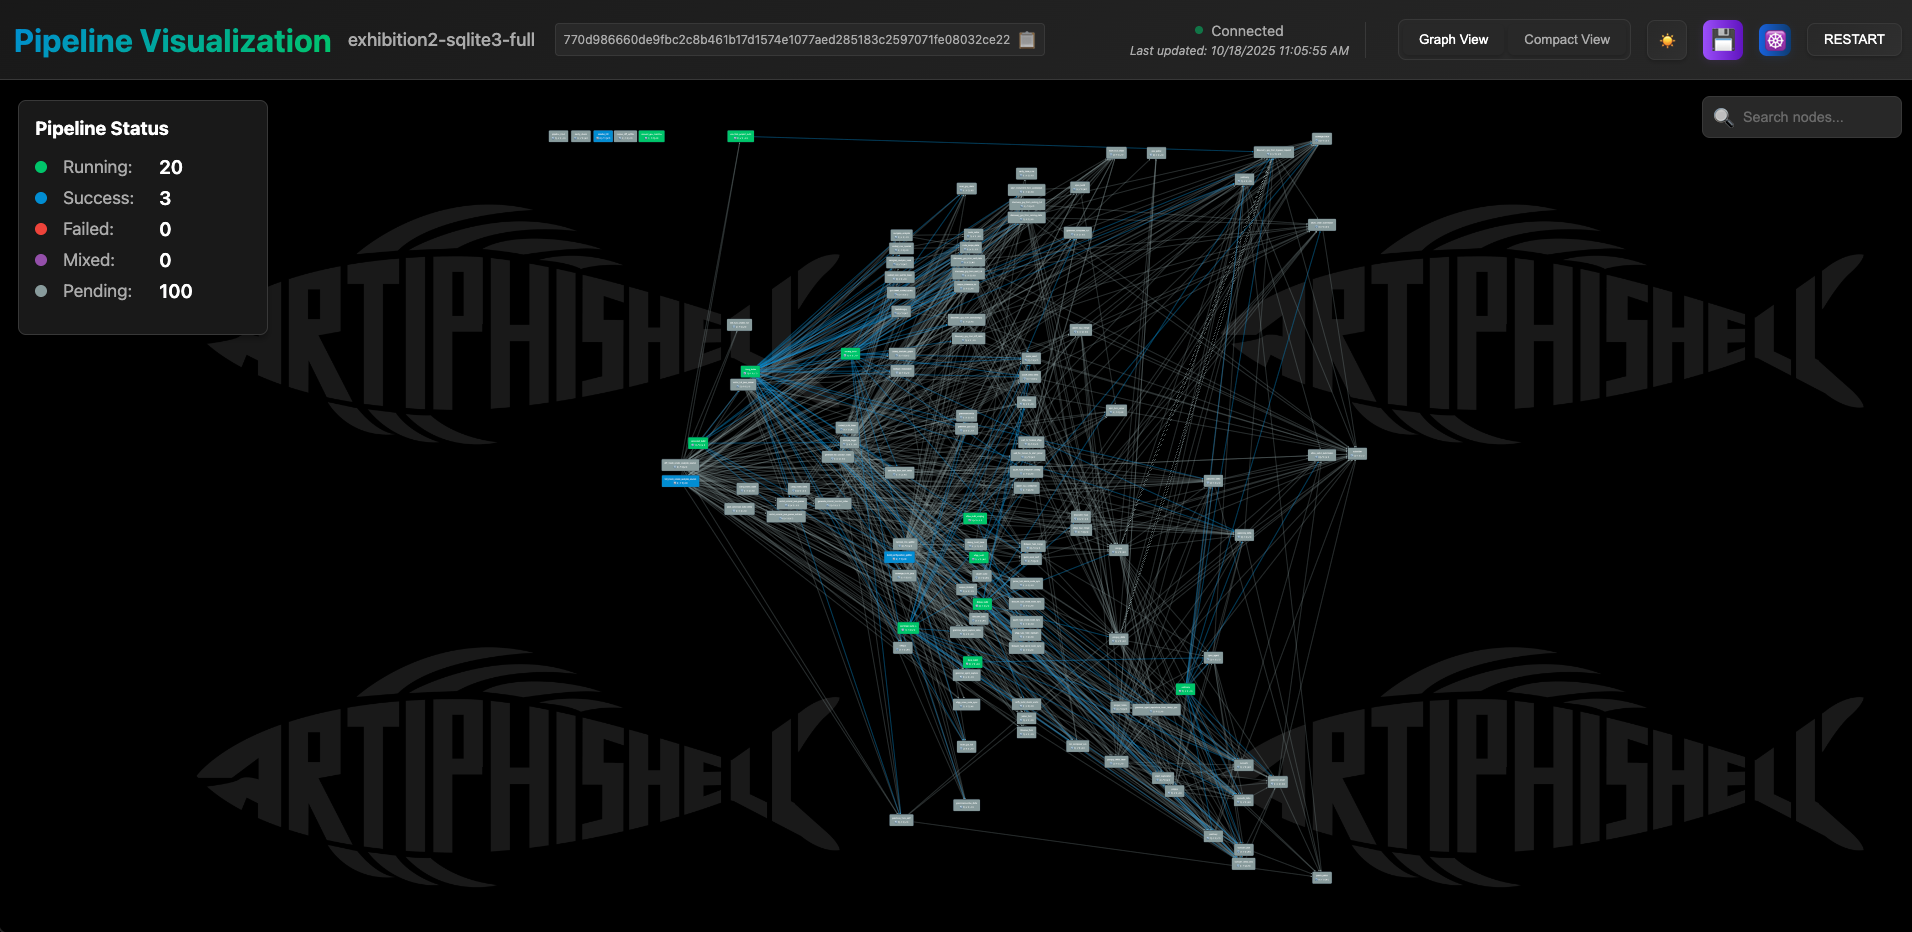
\includegraphics[width=\linewidth]{figures/pdviz.png}
  \caption{The \orchestrator's monitoring interface.}
  \label{fig:orchestrator}
\end{figure*}